\documentclass[10pt,brazil,english]{article}
\usepackage{amsfonts}
\usepackage{infocomp}
\usepackage{times}
\usepackage{amsmath}
\usepackage{amssymb}
\usepackage[T1]{fontenc}
\usepackage[english, portuguese]{babel}
\addto\captionsportuguese{
\renewcommand{\figurename}{Figura}
\renewcommand{\tablename}{Tabela}
\renewcommand{\refname}{REFER\^{E}NCIAS}
}
\usepackage[utf8]{inputenc}
\usepackage{multirow}
\usepackage{lscape}
\usepackage{rotating}
\usepackage{setspace} % espacamento entre linhas
\usepackage[table,xcdraw]{xcolor}
\usepackage{scalefnt}
\usepackage{graphicx}
\usepackage{hyperref}
\usepackage{subfigure}
\usepackage{enumerate}
\usepackage{caption}
\usepackage[sort,compress]{cite}
\usepackage[alf,abnt-repeated-author-omit=yes,abnt-etal-list=0]{abntex2cite}	% Citações padrão ABNT
%%%%%%%%%%%%%%%%%%%%%%%%%%%%%%%%%%%%%%%%%%%%%%%%%%%%%%%%%
\usepackage{fancyhdr}
\usepackage{mathtools}
\setcounter{page}{1}
\fancyhead{ }
\lhead{}
\chead{\footnotesize SIMULAÇÃO COMPUTACIONAL DE PROCESSOS EVOLUTIVOS E SELEÇÃO NATURAL}
\rhead{}
\cfoot{}
\rfoot{\thepage}%Direita do Rodapé
\renewcommand{\headrulewidth}{1pt}% Traço horizontal no cabeçalho

%%%%%%%%%%%%%%%%%%%%%%%%%%%%%%%%%%%%%%%%%%%%%%%%%%%%%%%%%

\usepackage{rangecite}

%\hyphenation{po-pu-la-ri-za-ção re-gis-tros do-mi-na-do-ra vio-la pe-ram-bu-lam dou-tri-na-ria-men-te co-nhe-ce-rem Ad-mis-tra-ção fa-bri-car so-cie-da-de in-fe-rio-res vee-men-te-men-te si-tua-ção pon-tuais}

\sloppy
\renewcommand{\captionfont}{\footnotesize}
\renewcommand{\captionlabelfont}{\footnotesize \bfseries}
\newtheorem{exemplo}{Exemplo}
\title{SIMULAÇÃO COMPUTACIONAL DE PROCESSOS EVOLUTIVOS E SELEÇÃO NATURAL}

\address{
$^{1}$Fundação Getulio Vargas (FGV)}

\author{Lucas Emanuel Resck Domingues$^{1}$}

\selectlanguage{english}

\abstract{This assignment aims to computationally simulate biological phenomena relevant to Evolution Theory, especially with regard to natural selection. The implementation of the simulation was made in \textit{Python} through \textit{Jupyter Notebook}. Resources competitive environments were implemented, and individuals, with their own characteristics, compete there. The characteristics may favor or disfavor the adaptation of the individual to the environment. Very adapted individuals survive and reproduce, passing on their characteristics to its descendents, sometimes with mutation. The results (that are somewhat intuitive) are compared, and hypothesis are made in a try to understand them.}

\keywords{Evolution. Natural Selection. Simulation. Python. Jupyter.}

\selectlanguage{brazil}

\resumo {Este trabalho visa simular computacionalmente fenômenos biológicos pertinentes à Teoria Evolutiva, principalmente no que diz respeito à seleção natural. A implementação da simulação foi realizada na linguagem \textit{Python} através de \textit{Jupyter Notebook}. Foram implementados ambientes de competição de recursos entre indivíduos, com características próprias, que favorecem ou desfavorecerem sua adaptação ao ambiente. Indivíduos bem adaptados sobrevivem e se reproduzem, repassando essas características aos seus descendentes, às vezes com mutações. Os resultados (intuitivos, de certa forma) são comparados, e hipóteses são formuladas na tentativa de compreendê-los.}

\palchaves{Evolução. Seleção Natural. Simulação. Python. Jupyter.}

\begin{document}
    \pagestyle{fancy} % CABECALHOO
    
    \maketitle
    \newpage
    
    \section{\uppercase{Introdução}}
    
    A teoria evolutiva é uma das teorias científicas melhor consolidadas no campo da Biologia. Em geral, em quase todo problema biológico pode-se identificar uma interseção com o campo evolutivo. Dessa forma, entender a evolução e os mecanismos de seleção natural é fundamental para que quaisquer estudos e pesquisas em Biologia possam ser desenvolvidos.
    
    O presente trabalho visa demonstrar a implementação de ambientes competitivos, com recursos escassos e seleção natural, para que se verifique, através de simulações computacionais, a adaptação de indivíduos de determinada espécie, no que diz respeito às características importantes para essa adaptação. Indivíduos, portanto, nascem, competem por recursos e talvez se reproduzam, assexuada ou sexuadamente. Além disso, podem gerar mutações nos seus descendentes. E, claro, morrem.
    
    Grande parte da estrutura dos ambientes implementados foi inspirada em alguns ambientes já implementados por \citeonline{Primer2018}, em sua série de vídeos exemplificando conceitos evolutivos.
    
    Esta é uma tarefa avaliada para a disciplina Modelagem de Fenômenos Biológicos, do curso de Matemática Aplicada da Fundação Getulio Vargas.
    
    \section{\uppercase{Metodologia}}
    
    A implementação dos ambientes competitivos foi realizada em \textit{Jupyter Notebook}, com a linguagem de programação \textit{Python}.
    
    Foram implementados três ambientes competitivos diferentes, que, na ordem em que são apresentados, representam a evolução de um modelo.
    
        \subsection{Ambiente com uma característica e reprodução assexuada}
        
        São criados vários indivíduos idênticos, cada um deles tendo característica de velocidade (no início, igual para todos). Além disso, os indivíduos possuem um grau de adaptação (\textit{fitness}), que, neste ambiente, é a própria velocidade. Sendo assim, quando mais veloz é um indivíduo, melhor adaptado ele está.
        
        O ambiente possui recursos de comida limitados. A distribuição dessas comidas em um período de tempo chamado dia é feita uma a uma (em rodadas), até que todas as comidas sejam distribuídas ou não tenha mais indivíduos capazes de recebê-las neste dia. Além disso, a distribuição aos indivíduos ocorre de acordo com probabilidades proporcionais aos graus de adaptação dos indivíduos. Portanto, indivíduos melhor adaptados têm maiores probabilidades de conseguir comida.
        
        Indivíduos têm energia, e cada rodada de distribuição consome uma parte da energia, parte esta afetada pela característica de velocidade. Neste ambiente, a cada rodada de distribuição, os indivíduos que estiverem buscando por comida têm subtraídos de sua energia o valor de sua velocidade ao quadrado. Ou seja, é possível que, em um determinado dia, um indivíduo não participe das rodadas finais de distribuição da comida, por exemplo.
        
        Se um indivíduo consegue uma comida, ele sobrevive para o próximo dia. Se ele consegue duas comidas, ele sobrevive para o próximo dia e se reproduz assexuadamente: quem nasce é um clone, porém com uma probabilidade de mutação na característica da velocidade. Aqueles indivíduos que não conseguem nenhuma comida até o fim da distribuição no dia morrem e não participam dos próximos dias.
        
        Todo esse processo ocorre durante vários dias.
        
        Durante a implementação, podem ser escolhidas algumas características do processo: velocidade inicial, quantidade inicial de comida, energia inicial, probabilidade de mutação, número de dias.
        
        Os ambientes foram testados com alguns parâmetros diferentes para verificar como a população de indivíduos se comporta diante desses parâmetros.
        
        \subsection{Ambiente com várias características, morte por idade e reprodução assexuada}
        
        Este ambiente tem algumas poucas diferenças em relação ao anterior. Além da característica de velocidade, os indivíduos possuem peso e tamanho. Agora, o grau de adaptação é o resultado da soma dessas três características. Durante a reprodução (assexuada), cada um desses fatores pode sofrer mutação, independentemente dos outros.
        
        Em cada rodada de distribuição de comida, os indivíduos que participam têm descontados de sua energia o valor de sua velocidade ao quadrado, o valor de seu tamanho ao cubo e o valor do seu peso.
        
        Além disso, os seres morrem por idade, sendo esta idade determinada antes da simulação.
        
        \subsection{Ambiente com várias características, morte por idade e reprodução sexuada}
        
        Este ambiente é análogo ao anterior, modificado apenas para incluir a reprodução sexuada. Para isso, os indivíduos têm sexo, determinado aleatoriamente no início de sua vida.
        
        Aqueles seres que recebem duas comidas durante um dia são aqueles com a capacidade de se reproduzir durante esse dia.
        
        Entre os indivíduos capazes de se reproduzir, os seres melhor adaptados de um sexo se reproduzem com os melhor adaptados do outro. Como o número de seres capazes de se reproduzir em um determinado dia pode ser diferente entre os sexos, pode haver indivíduos que não se reproduzem, mas são capazes disso, nesse dia.
        
        O indivíduo resultado do cruzamento de dois seres tem suas características iguais às médias aritméticas das características dos seus pais, com uma probabilidade de mutação em cada fator: velocidade, tamanho e peso.
    
    \section{\uppercase{Resultados}}
    
        \subsection{Ambiente com uma característica e reprodução assexuada}
        
        A Figura \ref{Fig1} mostra um gráfico da média dos graus de adaptação dos indivíduos no tempo, em dias, para uma simulação com os seguintes parâmetros: 100 indivíduos, inicialmente com velocidade 2, cada um com energia igual a 100, uma probabilidade de mutação de 0,5\%, durante 1000 dias e com 50 comidas disponíveis. Por exemplo, se escolhermos no eixo do tempo 300 dias, obtemos que a média dos graus de adaptação dos indivíduos no dia 300 é aproximadamente 0,4.
        
        Para a mesma simulação, as Figuras \ref{Fig2} e \ref{Fig3} apresentam o desvio padrão dos graus de adaptação dos indivíduos e o número de indivíduos no tempo.
        
        \begin{figure}[!hbtp]
            \begin{center}
                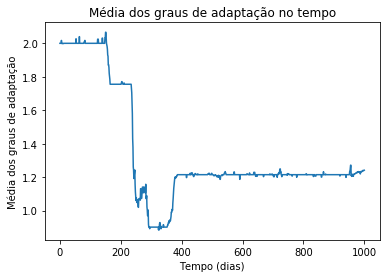
\includegraphics[scale=0.5]{Images/1-1.png}
            \end{center}
            \caption{Resultados da média dos graus de adaptação dos indivíduos no tempo na primeira simulação no primeiro ambiente.}
            \label{Fig1}
        \end{figure} 
        
        \begin{figure}[!hbtp]
            \begin{center}
                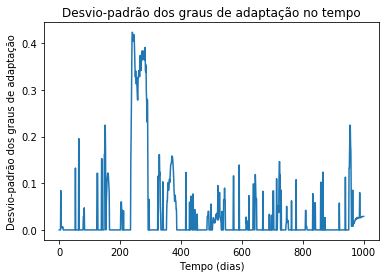
\includegraphics[scale=0.5]{Images/1-2.png}
            \end{center}
            \caption{Resultados do desvio-padrão dos graus de adaptação dos indivíduos no tempo na primeira simulação no primeiro ambiente.}
            \label{Fig2}
        \end{figure} 
        
        \begin{figure}[!hbtp]
            \begin{center}
                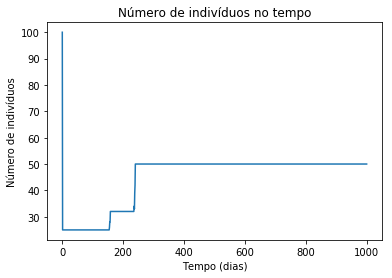
\includegraphics[scale=0.5]{Images/1-3.png}
            \end{center}
            \caption{Resultados do número de indivíduos no tempo na primeira simulação no primeiro ambiente.}
            \label{Fig3}
        \end{figure}
        
        Observamos que a média dos graus de adaptação tende a se estabelecer em 1,2, com baixo desvio-padrão. Além disso, o número de indivíduos se mantém constante em 50 a partir de certo dia.
        
        As Figuras \ref{Fig4}, \ref{Fig5} e \ref{Fig6} mostram, respectivamente, gráficos da média dos graus de adaptação dos indivíduos, do desvio-padrão dos graus de adaptação dos indivíduos e do número de indivíduos, todos no tempo, em dias, para uma simulação com os seguintes parâmetros: 100 indivíduos, inicialmente com velocidade 0,5, cada um com energia igual a 100, uma probabilidade de mutação de 0,5\%, durante 1000 dias e com 50 comidas disponíveis. Ou seja, com uma velocidade inicial de cada indivíduo bem menor do que na primeira simulação.
        
        \begin{figure}[!hbtp]
            \begin{center}
                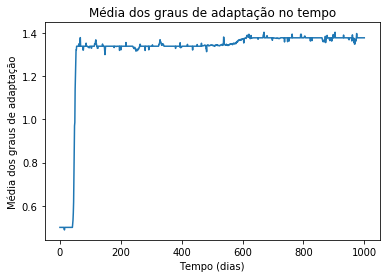
\includegraphics[scale=0.5]{Images/1-4.png}
            \end{center}
            \caption{Resultados da média dos graus de adaptação dos indivíduos no tempo na segunda simulação no primeiro ambiente.}
            \label{Fig4}
        \end{figure} 
        
        \begin{figure}[!hbtp]
            \begin{center}
                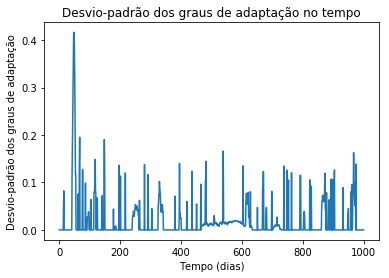
\includegraphics[scale=0.5]{Images/1-5.png}
            \end{center}
            \caption{Resultados do desvio-padrão dos graus de adaptação dos indivíduos no tempo na segunda simulação no primeiro ambiente.}
            \label{Fig5}
        \end{figure} 
        
        \begin{figure}[!hbtp]
            \begin{center}
                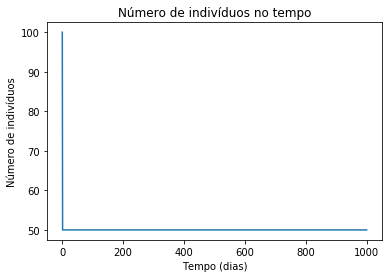
\includegraphics[scale=0.5]{Images/1-6.png}
            \end{center}
            \caption{Resultados do número de indivíduos no tempo na segunda simulação no primeiro ambiente.}
            \label{Fig6}
        \end{figure}
        
        Nesta segunda simulação, podemos notar que a média dos graus de adaptação também tende a um valor, neste caso 1,4, próximo ao da simulação anterior. Além disso, o número de indivíduos também se mantém em 50.
        
        Note que nas duas simulações neste ambiente os valores para os quais a média dos graus de adaptação se aproximam são, entre si, próximos.
        
        \subsection{Ambiente com várias características, morte por idade e reprodução assexuada}
        
        Para essa simulação, foram escolhidos os seguintes parâmetros: 100 indivíduos, velocidade, tamanho e peso iniciais iguais a 2, energia igual a 100, probabilidade de mutação de 0,5\%, idade de morte de 10 dias, durante  5000 dias, com 50 comidas disponíveis.
        
        As Figuras \ref{Fig7}, \ref{Fig8} e \ref{Fig9} apresentam a média das caracerísticas (velocidade, tamanho e peso) e do grau de adaptação, o desvio-padrão desses fatores e o número de indivíduos, respectivamente, todos no tempo, medido em dias.
        
        \begin{figure}[!hbtp]
            \begin{center}
                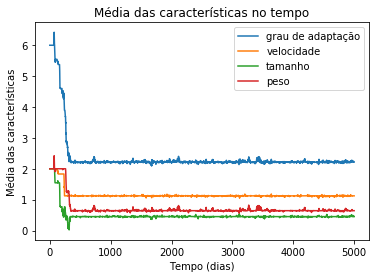
\includegraphics[scale=0.5]{Images/2-1.png}
            \end{center}
            \caption{Resultados da média das características dos indivíduos no tempo na primeira simulação no segundo ambiente.}
            \label{Fig7}
        \end{figure} 
        
        \begin{figure}[!hbtp]
            \begin{center}
                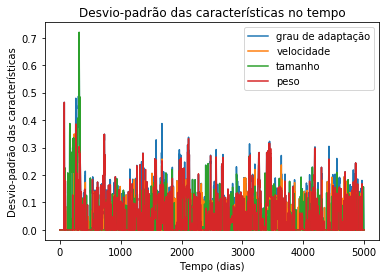
\includegraphics[scale=0.5]{Images/2-2.png}
            \end{center}
            \caption{Resultados do desvio-padrão das características dos indivíduos no tempo na primeira simulação no segundo ambiente.}
            \label{Fig8}
        \end{figure} 
        
        \begin{figure}[!hbtp]
            \begin{center}
                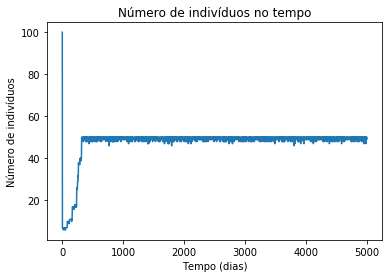
\includegraphics[scale=0.5]{Images/2-3.png}
            \end{center}
            \caption{Resultados do número de indivíduos no tempo na primeira simulação no segundo ambiente.}
            \label{Fig9}
        \end{figure}
        
        Logo no início da simulação, todas as características, e consequentemente o grau de adaptação, tendem a um valor. Com baixos desvios-padrões, velocidade se mantém pŕoxima de 1,1, tamanho se mantém em torno de 0,5 e peso, por sua vez, 0,6. Sendo assim, o grau de adaptação tende a ficar próximo de 2,2. O número de indivíduos também fica próximo de 50, porém não é mais constante, como nas simulações anteriores.
        
        As Figuras \ref{Fig10}, \ref{Fig11} e \ref{Fig12} mostram gráficos, respectivamente, da média das características e do grau de adaptação, do desvio-padrão desses fatores, e do número de indivíduos, todos no tempo, em dias, para uma simulação com os seguintes parâmetros: 100 indivíduos, velocidade, tamanho e peso iniciais iguais a 0,1, energia igual a 100, probabilidade de mutação de 0,5\%, idade de morte de 10 dias, durante  5000 dias, com 50 comidas disponíveis. As características iniciais dos indivíduos são bem menores do que na primeira simulação neste ambiente.
        
        \begin{figure}[!hbtp]
            \begin{center}
                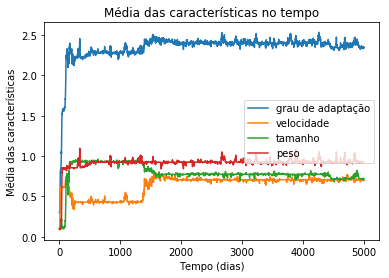
\includegraphics[scale=0.5]{Images/2-4.png}
            \end{center}
            \caption{Resultados da média das características dos indivíduos no tempo na segunda simulação no segundo ambiente.}
            \label{Fig10}
        \end{figure} 
        
        \begin{figure}[!hbtp]
            \begin{center}
                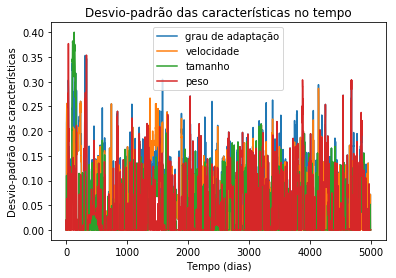
\includegraphics[scale=0.5]{Images/2-5.png}
            \end{center}
            \caption{Resultados do desvio-padrão das características dos indivíduos no tempo na segunda simulação no segundo ambiente.}
            \label{Fig11}
        \end{figure} 
        
        \begin{figure}[!hbtp]
            \begin{center}
                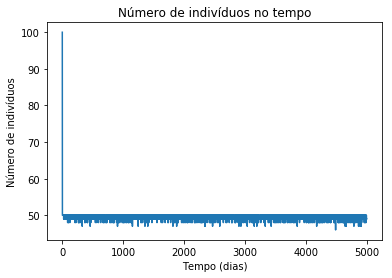
\includegraphics[scale=0.5]{Images/2-6.png}
            \end{center}
            \caption{Resultados do número de indivíduos no tempo na segunda simulação no segundo ambiente.}
            \label{Fig12}
        \end{figure}
        
        Com desvios-padrões um pouco mais altos, a velocidade e o tamanho procuram se manter perto de 0,7, e o peso, 0,9. Portanto, o grau de adaptação se mantém em torno de 2,3. Observe que, como na simulação na anterior, o número de indivíduos se mantém próximo de 50, porém não constante.
        
        Nas duas simulações, os valores para os quais as médias dos graus de adaptação se tornam próximos são entre si próximos.
        
        \subsection{Ambiente com várias características, morte por idade e reprodução sexuada}
        
        Foram escolhidos os parâmetros: 100 indivíduos, velocidade, tamanho e peso iniciais iguais a 1,2, energia igual a 100, probabilidade de mutação de 0,5\%, idade de morte de 10 dias, durante  5000 dias, com 50 comidas disponíveis.
        
        As Figuras \ref{Fig13}, \ref{Fig14} e \ref{Fig15} apresentam a média das caracerísticas (velocidade, tamanho e peso) e do grau de adaptação, o desvio-padrão desses fatores e o número de indivíduos, respectivamente, todos no tempo, medido em dias.
        
        \begin{figure}[!hbtp]
            \begin{center}
                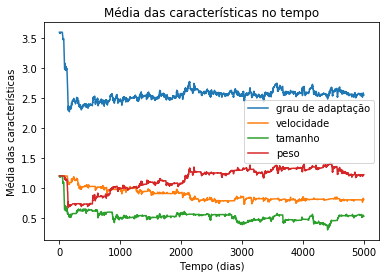
\includegraphics[scale=0.5]{Images/3-1.png}
            \end{center}
            \caption{Resultados da média das características dos indivíduos no tempo na primeira simulação no terceiro ambiente.}
            \label{Fig13}
        \end{figure} 
        
        \begin{figure}[!hbtp]
            \begin{center}
                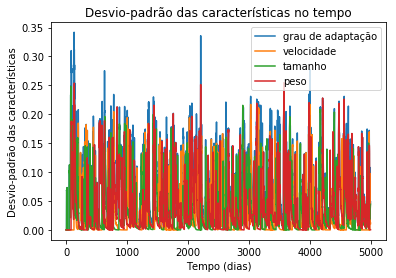
\includegraphics[scale=0.5]{Images/3-2.png}
            \end{center}
            \caption{Resultados do desvio-padrão das características dos indivíduos no tempo na primeira simulação no terceiro ambiente.}
            \label{Fig14}
        \end{figure} 
        
        \begin{figure}[!hbtp]
            \begin{center}
                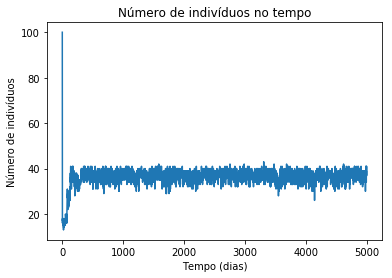
\includegraphics[scale=0.5]{Images/3-3.png}
            \end{center}
            \caption{Resultados do número de indivíduos no tempo na primeira simulação no terceiro ambiente.}
            \label{Fig15}
        \end{figure}
        
        Observamos que as características tendem a se tornar um pouco menos constantes. A velocidade se mantém perto de 0,8, tamanho se mantém em torno de 0,5 e peso, por sua vez, 1,2. Sendo assim, o grau de adaptação tende a ficar próximo de 2,6. O número de indivíduos fica próximo de 40, de forma não constante
        
        As Figuras \ref{Fig16}, \ref{Fig17} e \ref{Fig18} mostram gráficos da média das características e do grau de adaptação, do desvio-padrão desses fatores, e do número de indivíduos, respectivamente. Esses fatores variam no tempo, em dias, e foram considerados os seguintes parâmetros: 100 indivíduos, velocidade, tamanho e peso iniciais iguais a 0,1, energia igual a 100, probabilidade de mutação de 0,5\%, idade de morte de 10 dias, durante  5000 dias, com 50 comidas disponíveis.
        
        \begin{figure}[!hbtp]
            \begin{center}
                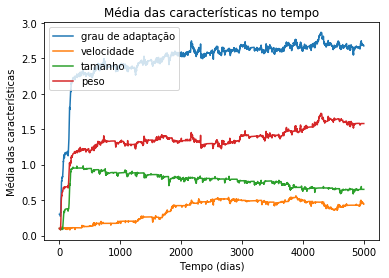
\includegraphics[scale=0.5]{Images/3-4.png}
            \end{center}
            \caption{Resultados da média das características dos indivíduos no tempo na segunda simulação no terceiro ambiente.}
            \label{Fig16}
        \end{figure} 
        
        \begin{figure}[!hbtp]
            \begin{center}
                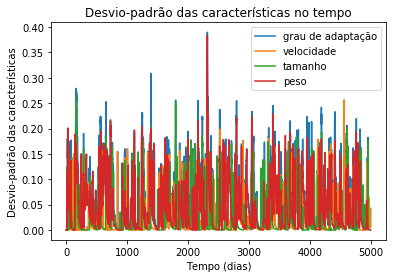
\includegraphics[scale=0.5]{Images/3-5.png}
            \end{center}
            \caption{Resultados do desvio-padrão das características dos indivíduos no tempo na segunda simulação no terceiro ambiente.}
            \label{Fig17}
        \end{figure} 
        
        \begin{figure}[!hbtp]
            \begin{center}
                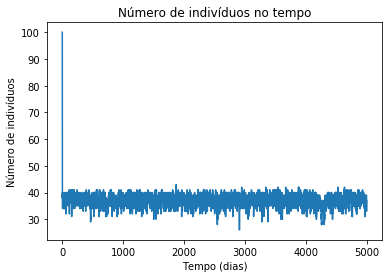
\includegraphics[scale=0.5]{Images/3-6.png}
            \end{center}
            \caption{Resultados do número de indivíduos no tempo na segunda simulação no terceiro ambiente.}
            \label{Fig18}
        \end{figure}
        
        A velocidade se mantém em torno de 0,4, o tamanho, 0,65, e o peso, 1,6, resultando em um grau de adaptação perto de 2,7. A população não é constante, em torno de 40 indivíduos.
        
        Como nos ambientes anteriores, os valores, nas duas simulações, para os quais as médias dos graus de adaptação tenderam são próximos entre si.
    
    \section{\uppercase{Considerações Finais}}
    
        Algo curioso é o número de indivíduos ficar, se não constante, pelo menos próximo a 50 (como na Figura \ref{Fig3}), que foi a quantidade de comida disponível escolhida em todas as simulações. Porém, há uma explicação bem direta. Considerando o primeiro ambiente, sem morte e com reprodução assexuada: se há comida para, no máximo, 50 indivíduos, não haverá mais indivíduos do que isso. Supondo que todos os 50 indivíduos têm comida, menos um deles, essa comida é entregue a um outro indivíduo, que acumula duas comidas e se reproduz, mantendo a população constante em 50. Esse raciocínio simples, porém, não é sempre verdade, pois pode haver a possibilidade de nenhum indivíduo participar da última rodada, por exemplo, pois todos estão sem energia ou já conseguiram duas comidas. Nos outros ambientes, esse raciocínio realmente não se aplica: há mortes por idade durante o processo. Ainda mais, no terceiro ambiente, que tem reprodução sexuada, se o número de indivíduos capazes de se reproduzir variar entre os sexos, alguns indivíduos capazes (que receberam duas comidas) não vão se reproduzir. Observemos a não constância do número de indivíduos no tempo, que inclusive se aproxima pouco do valor 50, na Figura \ref{Fig15}. 
    
        Em todas as simulações em todos os ambientes, a média dos graus de adaptação, no tempo, tende a um valor que aparenta ser ótimo ou pelo menos muito bom. Mais do que isso: em um mesmo ambiente, em simulações com parâmetros parecidos, porém com características iniciais diferentes, a média dos graus de adaptação tende a valores próximos. Ou seja, esse valor ótimo, ou pelo menos muito bom, não depende das características iniciais da simulação.
        
        Vamos considerar o primeiro ambiente (com apenas característica de velocidade): nas duas simulações a média dos graus de adaptação tendem a algo entre 1,2 e 1,4, como podemos verificar nas Figuras \ref{Fig1} e \ref{Fig4}, respectivamente. Na primeira simulação, o valor inicial é 2, e, na segunda, 0,5. Esse valor ótimo, ou pelo menos muito bom, para a característica pode ser interpretado com o valor de velocidade que maximiza o grau de adaptação em conjunto com o número de rodadas de distribuição de comida que o indivíduo vai participar (lembrando que a velocidade afeta a energia descontada em cada rodada).
        
        Podemos pensar: uma velocidade baixa, no primeiro ambiente, significa baixo grau de adaptação, porém muitas rodadas de distribuição; alta velocidade, por sua vez, significa alto grau de adaptação, mesmo que permitindo que o indivíduo participe de um número menor de rodadas.
        
        Qual seria uma hipótese razoável de por que um valor de velocidade entre 1,2 e 1,4 nesse primeiro ambiente? Considerando que o número de rodadas de distribuição de comida é 50 e a energia dos indivíduos é 100, para que ele participe de todas as rodadas de distribuição o desconto em cada rodada precisa ser igual a 2. Como o desconto é o quadrado da velocidade, basta que a velocidade seja aproximadamente 1,4. Esse valor, portanto, garante que todos os 50 indivíduos participem de todas as rodadas, com grau de adaptação máximo seguindo esse critério.
        
        Em todas as simulações, principalmente nas iniciais, é possível ver uma tendência de diminuição do desvio-padrão das características no tempo, mesmo que essa inclinação seja pequena e que o próprio desvio-padrão seja pequeno.
        
        Foram apresentados três modelos, ordenados por complexidade, de maneira crescente. O primeiro modelo, muito simples, após a convergência da média dos graus de adaptação, tende a manter esse valor durante o tempo, sem oscilações (veja a Figura \ref{Fig1}. Já no último modelo, essa convergência não é tão fácil de ser reconhecida, e a média dos graus de adaptação oscila em torno de um valor não trivial de ser estimado (veja a Figura \ref{Fig16}). Isso é esperado, pois, intuitivamente, tendemos a considerar que convergência está relacionada a simplicidade.
        
        Na verdade, a maioria dos, se não todos os, resultados apresentados são intuitivos, e demonstram o caráter algorítmico da seleção natural: indivíduos são diferentes devido aos cruzamentos e às mutações, e aqueles melhor adaptados são selecionados para perpertuar suas características, entre elas as que o tornam melhor adaptados.
    
    \bibliography{Referencias}
    
    \nocite{carykh2015}

\end{document} 